\chapter{Planning over Configuration Space Families}
\label{chap:family}

To this point,
we have considered motion planning problems in which a path is sought
within a fixed valid subset
$\mathcal{C}_{\ms{free}} \subset \mathcal{C}$
In Chapter~\ref{chap:lazysp},
we described a lazy search algorithm which is suited to domains in
which determining the weight of an edge
-- perhaps due to expensive set membership tests --
is expensive.
Chapter~\ref{chap:utility} discussed the concept of utility to
motion planning,
and showed examples of its application to single-query motion
planning problems.

However,
many applications exhibit structure beyond simple binary belief over
configuration validity.
In this chapter,
we introduce the \emph{family motion planning problem},
a generalization of the motion planning problem to a family of sets
over $\mathcal{C}$.
We then show how such a problem over familes can be represented
as in the utility function framework,
and given as input to the LEMUR motion planner described
in Chapter~\ref{chap:utility}.

This chapter proceeds as follows.
Section~\ref{sec:family:related-work} surveys related work.
In Section~\ref{sec:family:families-in-manipulation},
we motivate these the family motion planning problem
from the standpoint of manipulation tasks.
Section~\ref{sec:family:formulation} formulates the problem
generally.
We describe our approach in Section~\ref{sec:family:approach},
which details how the family problem can be represented
as a utility model that can be used by LEMUR.
The chapter concludes with experimental results on multi-step
manipulation tasks in Section~\ref{subsec:family:app-multi-step}.

\section{Related Work}
\label{sec:family:related-work}

The topic of reusing planning computation
between similar motion planning problems
has been extensively studied in the literature.
We include here a broad survey of existing approaches.
%the application sections
%(Section~\ref{subsec:family:app-multi-step}
%-- \ref{subsec:family:dynamic-environments}) also include
%relevant references to prior work.

\paragraph{Exact Algorithms.}
Exact planning methods construct explicit obstacles
directly in the configuration space.
Many such approaches allow for precomputation of primitives,
such as bitmaps \citep{kavraki1995cspacefft}
or C-space primitives for different workspace obstacles
\citep{newmanbranicky1991cspacetransforms}.
More recently,
Lien and Lu \citep{lien2009similarobstacles} describe a method to
build a PRM around obstacles in a database,
and then reposes them in a new world.
As described in Section~\ref{subsec:roadmaps:sensitive},
the exact approach is not easily applicable to articulated robots
with complex mappings from workspace to C-space.

\paragraph{Accommodating Dynamic Subsets in Sampling-Based Planning.}
Strong recent interest in sampling-based planning
has lead to the development of a number of approaches to handle
environments in which $\mathcal{C}_{\ms{free}}$ changes over time.
If a given discretization is asserted a priori,
this problem setting is similar to the dynamic shortest path problem
from Chapter~\ref{chap:ibid};
we refer the reader to that chapter for a review of related work.
Many sampling-based approaches attempt to prune and grow
the discretizations itself in response to these changes,
such as the Dynamic RRT \citep{ferguson2006drrt},
the Reconfigurable Random Forest (RRF)
\citep{li2002incrementalprmmanagement},
and the Lazy Reconfiguration Forest
\citep{gayle2007lazyreconfigforest}.
%We do the lazy thing as well (built into our planner).
%None of these reason about the structure of the configuration space.
However, these approaches do not reason explicitly about the
structure of the configuration space,
which we will consider
in Section~\ref{sec:family:families-in-manipulation}.

\paragraph{Considering Static and Dynamic Obstacles Separately.}
Some approaches do take advantage of such structure
through a two-level dichotomy between
the \emph{permanent} and \emph{non-permanent} configuration space
obstacles that induce $\mathcal{C}_{free}$.
Leven and Hutchinson \citep{leven2000changing, leven2002changing}
and similar work \citep{kallman2004dynamicroadmaps}
handle changing environments by
precomputing a self-collision-free roadmap offline,
and then pruning it at query time
using a mapping from workspace cells to roadmap edges.
%This can also be viewed through the multi-space lens
%-- I think this is just an instantiation of a bunch of sets.
%They're very focused on the precomputation stuff.
%However, this approach this can't directly handle grasped objects.
Other methods \citep{jaillet2004dynamicprm}
exploit the dichotomy between static and dynamic parts of
the world online.
The family motion planning problem is a generalization of these
formulations to more than two C-space subsets.

\paragraph{Task and Motion Planning.}
The structure in manipulation tasks that our approach leverages
is similar to the \emph{conditional reachability graph} which is
part of the recent \textsc{FFRob} heuristic task planning framework
\citep{garrett2014ffrob}.
While this framework does make use of a similar configuration
space decomposition for manipulation tasks
as described in Section~\ref{sec:family:families-in-manipulation},
it differs from our approach in two ways.
First,
it is concerned only with manipulation tasks,
and does not consider how the induced set of motion planning problems
can be formulated more generally
(e.g. in Section~\ref{sec:family:formulation}).
Second,
because the framework does not consider utility,
its motion planner is not able to exploit the configuration space
structure to the same extent as our approach.

%\subsection{Fast Collision Checking}
%
%Broad-phase collision checking.
%See Section~\ref{subsec:broad-phase} for more on this.
%I need cites!

%\subsection{Sampling Strategies}
%
%Also Kurniawati and Hsu's
%\emph{Workspace-based Connectivity Oracle}
%\citep{kurniawati2008workconnoracle}
%which is a smart sampling strategy which considers workspace
%geometry to inform PRM sampling.
%Kurniawati has a bunch of other work on PRM fundamentals and sampling.
%I think our approach is complementary to a PRM sampling strategy.
%Or, you could do deterministic sampling
%\citep{lavalle2002gridprms} \citep{geraerts2002prmcomparison}.
%
%\subsection{Multi-Resolution Planning}
%
%\noindent
%\begin{itemize}
%\item S. Kambhampati 1986
%\item R. Steffens 2010
%\item S. Zickler 2010
%\item K. Gochev 2013
%\end{itemize}

%\subsection{Graph Search}

%Many graph-search approaches are relevant to planning in similar
%environments.
%Algorithms such as
%D* \citep{stentz1994dstar}
%or LPA* \citep{koenig2004lpastar}
%handle dynamically changing (or incrementally discovered) worlds.
%Experience graphs \citep{phillips2012egraphs} are a method to apply
%computation from previous graph-search planning queries
%to the current problem.

%\subsection{Other Related Work to Integrate}
%
%Symbolic planning frameworks.

\section{Motivation: Families in Manipulation Tasks}
\label{sec:family:families-in-manipulation}

Motion planning approaches that build graphs
in the collision-free subset of
configuration space as described in Chapter~\ref{chap:roadmaps},
e.g. the
PRM \citep{kavrakietal1996prm}
and RRT \citep{lavallekuffner1999rrt},
have proven promising
for high-dimensional articulated robotics problems
in unstructured environments.
These approaches devote a large amount of computational effort
testing configurations and paths for collision
via the free set indicator function
(Section~\ref{subsec:roadmaps:building-graphs}),
and multi-query planners can then reuse the resulting graph
for other queries in the same collision-free subset.

However,
for manipulation problems,
this subset of the robot's configuration space
is sensitive to the locations and shapes of
both people and objects in the environment,
as well as the robot itself.
It also depends on the shape and pose of any object
grasped by the robot.
Consider the table clearing task in
Figure~\ref{fig:family:herbbin-multistep-example}.
The robot's valid subset $\mathcal{C}_{\ms{free}}$
changes each time the object is grasped or released.
Over the course of a planning episode,
these changing subsets constitute a family of related sets over
$\mathcal{C}$.

\begin{marginfigure}
   \centering
   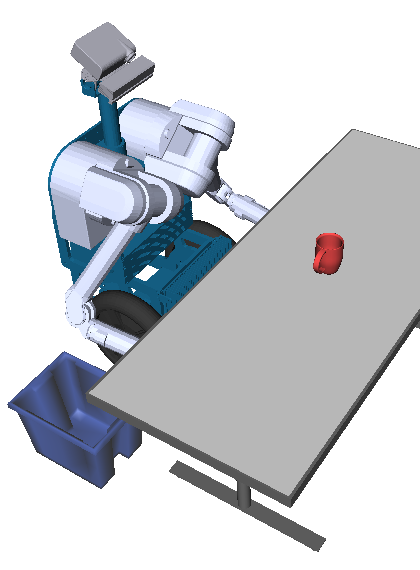
\includegraphics[width=2.5cm]{figs/herbbin/step0cropped.png}%
   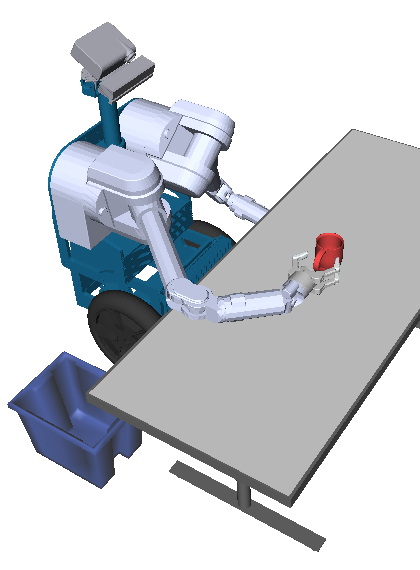
\includegraphics[width=2.5cm]{figs/herbbin/step01cropped.png}

   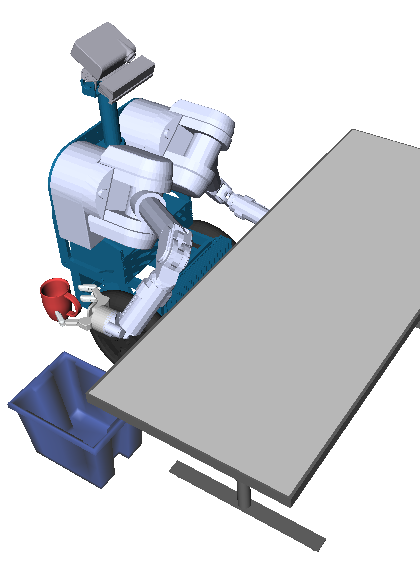
\includegraphics[width=2.5cm]{figs/herbbin/step12cropped.png}%
   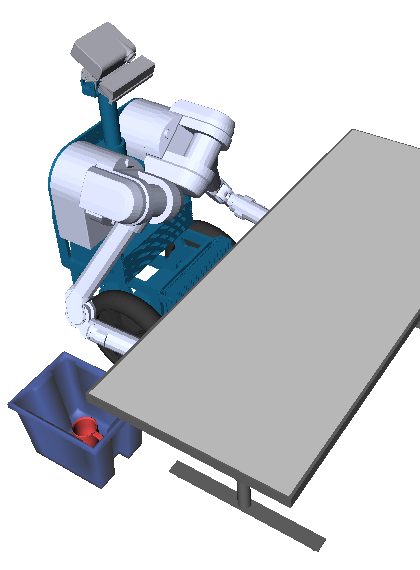
\includegraphics[width=2.5cm]{figs/herbbin/step2cropped.png}

   \caption{A simple manipulation task: retrieve the mug from
      the table, and drop it in the blue bin.
      This task requires plans in three distinct C-space free subsets.}
   \label{fig:family:herbbin-multistep-example}
\end{marginfigure}

This makes it difficult not only to apply the results of prior
planning computation to the current problem,
but also to efficiently consider multiple planned or hypothesized
motions,
since we must reconstruct our graph from scratch whenever
the environment changes.
This is especially the case for
multi-step manipulation tasks that must be planned into the future.
%We want to continuously update our representation for detours.

We use this multi-step manipulation task as a motivating example
for the family motion planning problem,
and dive more deeply next into the structure of the problem's
composite configuration space.
We will consider problems over other robots and applications
later in this chapter.

\subsection{The Composite Configuration Space}

The configuration of a quasistatic manipulation environment
with multiple moveable objects can be represented as a
\emph{composite configuration space},
\marginnote{The composite configuration space is also called
the \emph{joint configuration space}.}
consisting of the Cartesian product of the individual configuration
spaces of the constituent objects.
For example,
consider an environment with a robot $R$ and an object $O$;
each is endowed with a configuration space:
\begin{equation}
   \mathcal{C}_R \quad\mbox{and}\quad \mathcal{C}_O.
\end{equation}
For example,
the robot's configuration space may be represented as its joint angles,
while the object's configuration may be $SE(3)$.
The composite space is then defined as
\begin{equation}
   \mathcal{C}_{RO} = \mathcal{C}_R \times \mathcal{C}_O.
\end{equation}
Of course,
not all composite configurations will be feasible;
some may correspond to configurations in which the robot,
object, or static environment are intersecting each other (colliding),
while others may denote configurations of the object where it is
not at a stable placement or grasp configuration.

\paragraph{Visualizing the Composite Configuration Space.}
While the composite configuration space for any interesting
manipulation task
is of too high dimension to effectively visualize in full,
we can make an approximation shown
in Figure~\ref{fig:family:composite-volumes}.
Imagine that this 3D visualization represents a projection of
$\mathcal{C}_{RO}$
so that the two horizontal axes $x$ and $y$ correspond to
the robot's configuration space $\mathcal{C}_{R}$,
while the vertical axis $z$ corresponds to the object's
configuration space $\mathcal{C}_{O}$.
For the sake of this visualization,
we ignore constraints on feasible object placements.

\begin{figure}
   \centering
   \begin{tikzpicture}
      \node at (0,0) {\includegraphics{build/family-composite/plot-volumes}};
      \node at (5,0) {\includegraphics{build/family-composite/plot-volumes-individual}};
   \end{tikzpicture}
   \caption{Illustration of a composite configuration space
      for a manipulation task.}
   \label{fig:family:composite-volumes}
\end{figure}

Within the composite configuration space are three volumes
corresponding to composite configuration space obstacles,
shown individually at the right
of Figure~\ref{fig:family:composite-volumes}:
\begin{itemize}
\item First, in blue, is a volume which representing configurations
   in which the moveable object collides with the static environment.
   Note that the obstacle is invariant to the configuration of the robot.
\item Second, in green, is a volume in which the robot collides with
   the static environment.
   Similarly, note that this obstacle is invariant to the configuration
   of the object.
\item Third, colored by height, is a volume representing
   composite configurations in which the robot and object are colliding.
\end{itemize}
The manipulation problem can then be formulated as a motion planning
in this composite configuration space,
taking the system from a starting configuration
(e.g. with the robot in its home configuration, and the mug on the table
from Figure~\ref{fig:family:herbbin-multistep-example})
to a destination configuration(s)
(e.g. with the robot returned home, and the mug in the bin).
However,
this composite configuration space
is also encumbered by constraints which restrict allowable motion
to constraint manifolds.

\subsection{Transit and Transfer Manifolds}
The source of these constraint manifolds within the composite
configuration space is the fact that in prehensile manipulation tasks,
the moveable object cannot move on its own.
In fact,
any solution task alternates between two types of constraints:
\emph{transit} manifolds,
in which the robot's configuration changes while that of the object
remains constant,
and \emph{transfer} manifolds,
in which the configuration of the object moves as a function of
the robot's configuration (i.e. during a grasp).
(This dichotomy can be extended to multiple robots or
moveable objects.)
For an in-depth treatment of the structure of these manifolds
in manipulation tasks,
we refer the reader to \citep{simeon2004manipulation}.

\begin{figure*}
   \centering
   \begin{tikzpicture}
      \node at (0,0) {\includegraphics{build/family-composite/plot-ptop-manifold}};
      \node at (5.5,0) {\includegraphics{build/family-composite/plot-g-manifold}};
      \node at (11,0) {\includegraphics{build/family-composite/plot-pbottom-manifold}};
   \end{tikzpicture}
   \caption{Illustration of a transit and transfer constraint manifolds
      in the composite configuration space for a manipulation task,
      along with projections of each
      onto the robot's configuration space.}
   \label{fig:family:composite-manifolds}
\end{figure*}

\paragraph{Transit and Transfer Manifolds in $\mathcal{C}_{RO}$.}
To address a manipulation task, then,
the robot must move through this composite configuration space
$\mathcal{C}_{RO}$
while abiding by the underlying transit and transfer constraint
manifolds.
Consider the visualization
in Figure~\ref{fig:family:composite-manifolds},
with manifolds shown as red surfaces.
In the first step,
the robot must transit from its current configuration at left
to a grasp configuration at right,
while constrained to the transit manifold shown in red.
Next,
the second step is constrained to a transfer manifold
in which both the robot and the object move together
to an placement location.
Finally, the third step shows an addition transit away from
the placement location to a desired destination configuration.

\paragraph{Projecting Manifolds onto $\mathcal{C}_{R}$.}
Since the full composite configuration while constrained to a manifold
can be expressed as a function of the robot configuration $q_R$ only,
it is sufficient to consider eac subproblem as the projection of
the composite obstacles in $\mathcal{C}_{RO}$
onto the robot's configuration space $\mathcal{C}_{R}$.
Below each depiction of the manifolds
in Figure~\ref{fig:family:composite-manifolds}
lies a visualization of this projection,
along with the projected solution path.

The first and third subfigures correspond to transit subproblems,
in which motion through the composite space is constrained so that
the moveable object's configuration remains constant.
The second subfigure corresponds to a transfer subproblem,
in which the motion of the object directly follows from the
motion of the robot.

\subsection{Planning over a Family of Related Subsets}

The depictions of the three projections
in Figure~\ref{fig:family:composite-manifolds}
lends a concrete picture to the description of changing free subsets
depicted in Figure~\ref{fig:family:herbbin-multistep-example}.
Clearly,
when the composite configuration space $\mathcal{C}_{RO}$
is projected onto $\mathcal{C}_{R}$,
each of the three motion planning problems required by the task
induces a different free subset
$\mathcal{C}_{\ms{free}} \subset \mathcal{C}_{R}$.

Importantly however,
the free subsets are related.
In the visualized example,
the projection of the green composite obstacle is identical
across the three free subsets.

How can we take advantage of this?
Consider a roadmap method addressing the table clearing problem
in Figure~\ref{fig:family:herbbin-multistep-example}.
Suppose that a number of edges have already been evaluated in order
to find a valid path for the first step to grasp the red mug.
Once grasped, the active valid subset $\mathcal{C}_{\ms{free}}$
within which the second step must be planned has changed.
However,
any edge known to be valid for the previous step
can be validated in the new subset by simply checking the grasped
mug against the robot environment.
A similar example in a 2D world is presented
in Figure~\ref{fig:family:example}.

\begin{figure*}
   \begin{widepage}
   \begin{center}

   \subfloat[
      A two-part family problem in $\mathcal{C}$,
      first between $q_1$ and $q_2$ through $S_{12}$,
      then between $q_2$ and $q_3$ through $S_{23}$.
      The two free subsets $S_{12}$ and $S_{23}$ are distinct
      but related.
   ]{
      \includegraphics{build/figstar-a}
   }%
   \quad%
   \subfloat[
      The free subsets are related via other underlying
      subsets of $\mathcal{C}$, with $S_{12}=A \cap B$
      and $S_{23}=A \cap C$.
      A planner solving the first part (from $q_1$ to $q_2$)
      has found paths in $S_{12}$.
   ]{
      \label{subfig:family:figstar-intersections}
      \includegraphics{build/figstar-b}
   }%
   \quad%
   \subfloat[
      Due to the set relations,
      a planner solving the second part
      (from $q_2$ to $q_3$ in $S_{23}$)
      can reuse any segment known to be in $S_{12}$
      by checking only for its membership in $C$.
   ]{
      \includegraphics{build/figstar-c}
   }

   \vspace{0.1in}

   \subfloat[
      A forklift in a parking lot ($q_1$)
      must retrieve an object ($q_2$)
      and reverse park ($q_3$).
      This two-part problem
      requires plans in distinct collision-free
      $\mathcal{C}$-subsets
      $S_{12}$ and $S_{23}$.
   ]{%
      \begin{tabular}{c}
      \includegraphics{build/example-2d-a} \\
      \includegraphics{build/example-2d-b} \\
      \includegraphics{build/example-2d-c} \\
      \end{tabular}%
      \label{subfig:family:figstar-manip-probdef}
   }%
   \quad%
   \subfloat[
      Sets $S_{12}$ and $S_{23}$ are subsets of
      the configuration space of the robot $\mathcal{C}=\mbox{SE}(2)$,
      and can be represented as intersections
      of underlying subsets $A$, $B$, and $C$
      as in \protect\subref{subfig:family:figstar-intersections}.
   ]{%
      \label{subfig:family:figstar-manip-spaces}
      \begin{tabular}{c}
      \includegraphics{build/example-2d-d} \\
      \includegraphics{build/example-2d-e} \\
      \includegraphics{build/example-2d-f} \\
      \end{tabular}%
   }%
   \quad%
   \subfloat[
      After planning a path from $q_1$ to $q_2$ (top),
      a planner can reuse a configuration in $S_{12}$ (middle)
      by checking only for its membership in subset $C$,
      resulting in plan reuse (bottom).
   ]{%
      \begin{tabular}{c}
      \includegraphics{build/example-2d-g} \\
      \includegraphics{build/example-2d-h} \\
      \includegraphics{build/example-2d-i} \\
      \end{tabular}%
   }

   \caption[
      An illustration of a family motion planning
      problem in a common configuration space $\mathcal{C}$.
      The problem definition generalizes to an arbitrary number of
      configuration space subsets and set relations between them.
      When two queries in different subsets are solved sequentially,
      a family motion planner can reuse path segments less expensively.
      See Section~\ref{subsec:family:app-multi-step} for examples in
      manipulation.
   ][99in]{x}
   \label{fig:family:example}

   \end{center}
   \end{widepage}
   
   \vspace{0.1in}
   \smallskip\noindent\small Figure \ref{fig:family:example}:
   An illustration of a family motion planning
   problem in a common configuration space $\mathcal{C}$.
   The problem definition generalizes to an arbitrary number of
   configuration space subsets and set relations between them.
   When two queries in different subsets are solved sequentially,
   a family motion planner can reuse path segments less expensively.
   See Section~\ref{subsec:family:app-multi-step} for examples in
   manipulation.

\end{figure*}

This example from a simple manipulation task motivates
the formalization of the family motion planning problem
in Section~\ref{sec:family:formulation},
which is more generally applicable than manipulation tasks
in particular.
We then develop our intuition from the simple examples in this section
when describing our approach in greater detail
in Section~\ref{sec:family:approach}.

\section{The Family Motion Planning Problem}
\label{sec:family:formulation}

The family motion planning problem is
a generalization of both the movers' problem
(Section~\ref{chap:roadmaps})
and the \emph{multi-query} planning problem
\citep{kavrakietal1996prm}.
%The reader is referred to
%Figure~\ref{fig:family:example}
%for a general example,
%as well as a simple instantiation on a 2D manipulation task.
%which is discussed in more detail in
%Section~\ref{subsec:multi-prm-example}.
%The family problem formulation
%explicitly captures both planning and execution effort
%and can therefore be used as an ensemble effort model
%for use in the E$^8$-PRM planner across queries.
The problem is multi-query in
a fixed configuration space $\mathcal{C}$,
in that it accommodates multiple distinct motion planning queries
(e.g. between $q_{\ms{start}},q_{\ms{dest}} \in \mathcal{C}$).
However, unlike existing multi-query formulations in which all
queries demand solution paths contained within a single common subset of
$\mathcal{C}$
(i.e. the set of collision-free configurations, denoted
$\mathcal{C}_{\mbox{\scriptsize free}}$),
the family problem allows for the specification of
a \emph{family} of multiple such subsets
$\mathcal{F} = \{ A, B, \dots \}$.
Like $\mathcal{C}_{\mbox{\scriptsize free}}$,
each member of $\mathcal{F}$
is a subset of the common configuration space
(that is,
$S \subseteq \mathcal{C} \;\forall\; S \in \mathcal{F}$),
and each subset $S$ has its own indicator and planning estimator
${\bf 1}_S[\cdot]$ and $\hat{p}_S(\cdot)$
as in Section~\ref{subsec:roadmaps:building-graphs}.
For example,
in Fig.~\ref{fig:family:example}\subref{subfig:family:figstar-manip-spaces},
$\mathcal{C}$-subset $B$
consists of configurations
free of collision between the robot and
the initial object pose.

The problem supports an arbitrary number of queries $\mathcal{U}$.
Each query $u$ demands a solution path through a \emph{single}
$\mathcal{C}$-subset $U \in \mathcal{F}$
(see Fig~\ref{fig:family:query-to-subset}):
\begin{equation}
  u : ( q_{start},\; q_{goal},\; U ) .
  \label{eqn:family:q}
\end{equation}

\begin{marginfigure}
   \centering
   \subfloat[Multi-query planning]{
      \includegraphics{build/query-to-subset-a}
   }
   \vspace{-0.05in}
   \subfloat[Family motion planning]{
      \includegraphics{build/query-to-subset-b}
   }
   \vspace{0.1in}
   \caption{While queries in multi-query planning reference
     the same subset of $\mathcal{C}$,
     each family query references one of a number of such sets.}
   \label{fig:family:query-to-subset}
\end{marginfigure}

\begin{marginfigure}
   \centering
   \subfloat[Containment relation]{
      \begin{tabular}{cc}
      \includegraphics{build/relations-inclusion} \\
      $A \subseteq B$ \\
      \end{tabular}
      \label{fig:family:relations-containment}
   }
   \vspace{-0.05in}
   \subfloat[Intersection relation]{
      \begin{tabular}{cc}
      \includegraphics{build/relations-intersection} \\
      $A = B \cap C$ \\
      \end{tabular}
      \label{fig:family:relations-intersection}
   }
   \vspace{0.1in}
   \caption{Types of subset relations.
     Each relation can be expressed directly as set relations
     w.r.t a set $S$,
     or equivalently as logical statements
     on the corresponding indicator functions
     $\mathbf{1}_S(\cdot)$.}
   \label{fig:family:relations}
\end{marginfigure}

Finally, the family problem includes a list of set relations
$\mathcal{R}$
between the $\mathcal{C}$-subsets in $\mathcal{F}$.
These can be expressed directly using set theoretic relations,
or equivalently as logical statements
on the corresponding indicator functions.
Common types of such relations
(containment and intersection)
are illustrated in Fig.~\ref{fig:family:relations}.
Fig.~\ref{fig:family:example} gives an example of intersection relations;
an example of containment is a padded (conservative) robot model.

Together, these four elements
(a configuration space $\mathcal{C}$,
subsets $\mathcal{F}$ each with endowed indicators,
a set of queries $\mathcal{U}$,
and a list of subset relations $\mathcal{R}$)
comprise a family motion planning problem.

\paragraph{Revisiting the Example (as a Family Motion Planning Problem).}
Consider the diagram from Fig.~\ref{fig:family:example}.
$\mathcal{F}$ consists of five $\mathcal{C}$-subsets labeled
$A$, $B$, $C$, $S_{12}$, and $S_{23}$,
and we have two queries,
$u_{12}: (q_1, q_2, S_{12})$
and
$u_{23}: (q_2, q_3, S_{23})$.
$\mathcal{R}$ consists of the two relations
$S_{12} = A \cap B$ and $S_{23} = A \cap C$.
Suppose a cost model $\mathcal{M}$
wherein evaluating the indicator
$\mathbf{1}_A$ incurs cost 4,
evaluating $\mathbf{1}_B$ and $\mathbf{1}_C$ incurs cost 2,
and evaluating $\mathbf{1}_{S_{12}}$ and $\mathbf{1}_{S_{23}}$
incurs cost 6.
In the manipulation example in
Fig.~\ref{fig:family:example}\subref{subfig:family:figstar-manip-probdef},
this would be the case if each
pairwise outlined shape collision check incurs unit cost.

Suppose a graph structure within ${S_{12}}$ has been grown to solve
the first query $u_{12}$.
During the subsequent solve of query $u_{23}$,
an existing path segment known to be in ${S_{12}}$ can be shown to
also be contained within ${S_{23}}$ by only evaluating $\mathbf{1}_C$.
In the manipulation example,
reusing an a configuration from the previous search
would require only a check of cost 2,
instead of cost 6 for a new configuration.
Thus, we might hope that a planner may be biased towards reusing
said path segments in this case.

%\paragraph{Applications of the Family Motion Planning Problem.}
%So far,
%we have motivated the family motion planning problem
%for the application of manipulation planning tasks.
%However,
%the same structure is present in a number of other applications,
%including cached invariant geometry
%and conservative geometric approximations.
%We review these applications
%in Sections~\ref{subsec:family:app-multi-step}
%-- \ref{subsec:family:dynamic-environments}.

\section{Approach: A Utility Model over Family Beliefs}
\label{sec:family:approach}

Recall from Chapter~\ref{chap:utility}
that the LEMUR motion planner takes as input
a domain-specific ensemble cost model
$\mathcal{M}$ to provide it with planning and execution cost
estimates for prospective edges.
\marginnote{See Section~\ref{subsec:lemur:ensemble-edge-cost-models}
for the definition of an ensemble edge cost model.}
This allows it to exploit domain-specific
knowledge and structure that may be present.

We wish to capture the structure of the family motion planning problem
via such an ensemble edge cost model $\mathcal{M}_{\ms{family}}$.
To do so requires us to implement the remaining planning cost estimator
$\grave{p}_{\ms{family}}(e)$
as a function of the underly family
$\mathcal{F}$ of $\mathcal{C}$-subsets
and the intersection/inclusion relations between them.
We accomplish this over the course of a planning episode
by reasoning explicitly about belief over the subset membership
of individual configurations and edges.

%The model maintains
%(a) a family $\mathcal{F}$ of $\mathcal{C}$-subsets
%relevant to the problem,
%(b) the inclusion/intersection relations between them,
%and (c) the set of validity checks that have been performed
%for each edge.
%This knowledge enables it to implement an edge
%planning cost estimator $\grave{p}_{\ms{family}}(e)$
%which determines the minimum set of collision checks necessary
%to validate an edge within a target subset.

\subsection{Family Beliefs}

Consider a family $\mathcal{F}$ consisting of $n$ subsets,
and consider a configuration $q \in \mathcal{C}$ on which
we may have invoked one or multiple subset indicator functions.
\marginnote{Recall that for subset $S$,
invoking the indicator function $\mathbf{1}_S$
on configuration $q$
returns a binary value representing whether $q \in S$.}
How can we generally represent our knowledge
about the subset membership of $q$?
We can form a \emph{belief space} $\mathcal{B}$ as follows
\begin{equation}
   \mathcal{B} = \prod_{S \in \mathcal{F}}
      \{ \mbox{Unknown}, \mbox{False}, \mbox{True} \}.
   \label{eqn:family:beliefs}
\end{equation}
That is,
a belief state $b \in \mathcal{B}$ stores
knowledge of subset membership for each subset $S \in \mathcal{F}$.
(We will abbreviate the membership beliefs for each state
in (\ref{eqn:family:beliefs})
as U, F, and T respectively.)

\paragraph{Composing a Family Belief Graph.}
Consider the initial belief state of a configuration
$b_{\ms{init}} = \left( \mbox{U}, \mbox{U}, \dots \right)$
for all subsets.
How does a belief state $b$ transition after invoking a particular
indicator function?
In the most general case,
invoking the $i$-th indicator $\mathbf{1}_{S_i}$ returning
$r \in \{\mbox{F},\mbox{T}\}$
results in a belief state $b'$ equal to $b$ but with its
$i$-th component set to $r$.
(The existing $i$-th component of $b$ must either be U
or already be $r$ if the indicators are consistent.)
This simple transition model induces a directed
\emph{family belief graph}
$G_{\mathcal{F}} = (V_{\mathcal{F}}, E_{\mathcal{F}})$
where $V_{\mathcal{F}} = \mathcal{B}$
and each edge $e_{\mathcal{F}} \in E_{\mathcal{F}}$ represents $(S,r)$,
the result of invoking an available indicator function $\mathbf{1}_{S}$
and having it return the binary result $r$.

\begin{marginfigure}
   \centering
   \includegraphics{build/family-belief-graph-example}
   \caption{Example family belief graph
      for a family of two subsets, $S_1$ and $S_2$.
      From the initial belief $b_{\ms{init}} = (\mbox{U},\mbox{U})$,
      each transition $(S,r)$ represents invoking
      indicator $\mathbf{1}_S$ with returned binary result $r$.
      }
   \label{fig:family:belief-graph-example}
\end{marginfigure}

For example,
consider a family $\mathcal{F}$ consisting of two unrelated subsets,
$S_1$ and $S_2$.
The family belief graph $G_{\mathcal{F}}$
illustrated in Figure~\ref{fig:family:belief-graph-example}
shows all possible belief transitions on the graph.

\subsection{Subset Relations and the Family Belief Graph}
In a family motion planning problem,
the family of subsets $\mathcal{F}$
is accompanied by a set of subset relations $\mathcal{R}$.
These relations have implications on the family belief graph
$G_{\mathcal{F}}$.
To build the revised graph,
we convert both the belief state $b$
and the subset relations $\mathcal{R}$
into a set of \emph{logical propositions}.

\paragraph{Beliefs and Subset Relations as Logical Propositions.}
A logical proposition is a statement consisting of
propositional variables and logical operators.
We will use bolded letters to denote propositional variables.
A set of propositions $\mathcal{P}$ can be used as \emph{premises}
as part of an \emph{argument} to demonstrate a \emph{conclusion};
a logical solver can then be used validate or invalidate the argument.
For example, an argument with these premises and conclusion
$\{ (\mathbf{A} \Rightarrow \mathbf{B}), (\lnot\mathbf{B}) \}
\Rightarrow (\lnot\mathbf{A})$
can be shown to be valid.

Any belief state $b$ can be represented as a set of logical
propositions.
Consider again the simple family
from Figure~\ref{fig:family:belief-graph-example}
consisting of subsets $S_1$ and $S_2$
(with $S_i \subseteq \mathcal{C}$).
We will introduce the propositional variable $\mathbf{S}_i$ as follows:
for some query configuration $q \in \mathcal{C}$,
the proposition $\mathbf{S}_i$ implies $q \in S_i$,
whereas $\lnot\mathbf{S}_i$ implies $q \notin S_i$.
\marginnote{We keep distinct notation for the indicator
function predicate $\mathbf{1}_S$ over $\mathcal{C}$
and the corresponding propositional variable $\mathbf{S}$;
the former is used as a subroutine to be invoked to determine
subset membership,
whereas the latter is used to represent actual or hypothesized
assignments to the propositional logic engine.}
Therefore,
a belief state $b$ can be converted into a set of propositions
$\mathcal{P}_b$:
\begin{equation}
   \mathcal{P}_b = \{ \mathbf{S}_i \; \forall \; i \; | \; b[i] = \mbox{T} \}
      \cup \{ \lnot\mathbf{S}_i \; \forall \; i \; | \; b[i] = \mbox{F} \}.
   \label{eqn:family:belief-propositions}
\end{equation}
For example,
belief $b=(T,F)$ corresponds to
$\mathcal{P}_b = \{ \mathbf{S}_1, \lnot\mathbf{S}_2 \}$,
and belief $b=(U,U)$ corresponds to $\mathcal{P}_b = \emptyset$.

The set of subset relations $\mathcal{R}$
can also be represented as a set of propositions.
In particular,
the containment relation $A \subseteq B$
(Figure~\ref{fig:family:relations-containment})
yields $\{ ( \mathbf{A} \Rightarrow \mathbf{B} ) \}$
and the intersection relation $A = B \cap C$
(Figure~\ref{fig:family:relations-intersection})
yields 
$\{ ( \mathbf{B} \wedge \mathbf{C} \Rightarrow \mathbf{A} ),
( \mathbf{A} \Rightarrow \mathbf{B} ),
( \mathbf{A} \Rightarrow \mathbf{C} )
\}$.
Converting each relation in $\mathcal{R}$ in this way
yields an equivalent set of relational propositions
$\mathcal{P}_{\mathcal{R}}$.

\paragraph{Subset Relations Prune the Family Belief Graph.}
The relational propositions $\mathcal{P}_{\mathcal{R}}$
together with the belief propositions $\mathcal{P}_b$ for
each belief state $b$ given by (\ref{eqn:family:belief-propositions})
can then be used along with a propositional
logic engine to compute the family belief graph
for a particular family motion planning problem.
In particular,
consider a given belief state vertex $b \in V_{\mathcal{F}}$
and a proposed out-edge $(S,r)$.
Let $\mathcal{P}_e$,
the resulting additional set of propositions for this edge,
be $\{ \mathbf{S} \}$ if $r = \mbox{True}$,
or $\{ \lnot\mathbf{S} \}$ otherwise.
Then $i$-th component of the successor belief state $b'$
is formed by considering the following two propositional arguments:
\begin{equation}
   b'[i] = \left\{ \begin{array}{cl}
   \mbox{True}
      & \mbox{if }
      \mathcal{P}_{\mathcal{R}} \cup \mathcal{P}_b \cup \mathcal{P}_e
         \Rightarrow \mathbf{S}_i
      \mbox{ is valid} \\
   \mbox{False}
      & \mbox{if }
      \mathcal{P}_{\mathcal{R}} \cup \mathcal{P}_b \cup \mathcal{P}_e
         \Rightarrow \lnot\mathbf{S}_i
      \mbox{ is valid} \\
   \mbox{Unknown}
      & \mbox{otherwise.}
   \end{array} \right.
\end{equation}

\begin{marginfigure}
   \centering
   \includegraphics{build/family-belief-graph-example-wrels}
   \caption{Example family belief graph
      for a family of two subsets, $S_1$ and $S_2$,
      with the subset relation that $S_1 \subseteq S_2$.
      Compare this family belief graph
      to Figure~\ref{fig:family:belief-graph-example}
      without the relation.}
   \label{fig:family:belief-graph-example-wrels}
\end{marginfigure}

We show the effect of subset relations $\mathcal{R}$
on the family belief graph for our simple example family
with an additional containment relation
in Figure~\ref{fig:family:belief-graph-example-wrels}.
The additional proposition from $\mathcal{P}_{\mathcal{R}}$,
namely that $\mathbf{S}_1 \Rightarrow \mathbf{S}_2$,
prunes the original graph
in Figure~\ref{fig:family:belief-graph-example}
by removing inconsistent belief states and transitions.

We also illustrate the family belief graph
for the more complex family motion planning
problem in Figure~\ref{fig:family:example}.
Recall that the family $\mathcal{F}$ consists of
five $\mathcal{C}$-subsets, $A$, $B$, $C$, $S_{12}$, and $S_{23}$,
and $\mathcal{R}$ consists of the subset relations
$S_{12} = A \cap B$ and $S_{23} = A \cap C$.
The family belief graph is shown
in Figure~\ref{fig:family:appendix-suction-example-graph}
in Appendix~\ref{chap:appendix-family}.

\subsection{A Family Utility Model}

A key input to the LEMUR planner from Chapter~\ref{chap:utility}
is the ensemble edge cost model $\mathcal{M}$
which captures domain-specific estimates of both the
execution cost $\hat{x}$ and the remaining planning cost $\grave{p}$
for each edge on its roadmap.
How can we take advantage of our family belief graph
in order to implement such a model for the family
motion planning problem?

Recall that the formulation of the family motion planning problem
(Section~\ref{sec:family:formulation})
includes for each subset indicator function $\mathbf{1}_S$
an invocation cost estimate $\hat{p}_S$.
Our key insight is that our ensemble edge cost model
$\mathcal{M}_{\ms{family}}$ can
(a) maintain for each edge $e$ its current belief state $b_e$
within and between each planning query,
and (b) leverage the family belief graph
in order to compute for any current edge 
an optimistic optimal sequence of indicator function invocations
in order to demonstrate that the edge $e$ is a member of the
query subset $S_u$.

\paragraph{Beliefs from Configurations to Edges.}
Paramount in our approach is the ability to reason over edge beliefs.
So far in Section~\ref{sec:family:approach},
we have developed a family belief graph $G_{\mathcal{F}}$
informed by the set of subset relations $\mathcal{R}$
which allows us to reason about the evolution of our belief
over the subset memberships of a query configuration $q \in \mathcal{C}$.
Can we use this same belief graph to reason about edge beliefs as well?

While this is not generally true for arbitrary subset relations,
we can demonstrate that it is true for the particular relations that
we are considering -- namely, containments and intersections.
Consider the following definition
for a subset $S \subseteq \mathcal{C}$.
Consider an edge $e \in E$ which corresponds to a particular trajectory
$\xi_e : [0,1] \rightarrow \mathcal{C}$
as described in Chapter~\ref{chap:roadmaps}.
We will define edge set membership as:
\begin{equation}
   e \in S \iff \xi_e(t) \in S \;\;\forall\;\; t \in [0,1].
   \label{eqn:family:edge-subset-membership-defn}
\end{equation}
Consider the containment relation $A \subseteq B$;
it can be easily shown by (\ref{eqn:family:edge-subset-membership-defn})
that if $e \in A$, then $e \in B$.
A similar statement can be made about the intersection relation
$A = B \cap C$.
If $e \in A$, then $e \in B \cap C$ and vice versa.

\begin{marginfigure}
   \centering
   \begin{tabular}{cc}
      \includegraphics{build/relations-disjoint} \\
      $A = C \setminus B$ \\
   \end{tabular}
   \caption{A subset relation which does not carry over directly
      from configurations to edges.}
   \label{fig:family:relations-disjoint}
\end{marginfigure}

An example of a set relation for which the edge membership relations
do not follow directly from the configuration membership relations
is shown in Figure~\ref{fig:family:relations-disjoint}.
In this example,
the subset relation $A = C \setminus B$ implies that if $q \in A$,
then $q \notin B$.
However,
this is not true in general for edges.
Fortunately,
containment and intersection relations are sufficient for all
instances of family motion planning problems that we consider.

\paragraph{Computing an Optimistic Optimal Belief Policy.}
Using the invocation cost estimates $\hat{p}_S$
for each subset $S \in \mathcal{F}$,
we can create an edge weight function
$w_{\hat{p}} : E_{\mathcal{F}} \rightarrow \mathbb{R}$ as
\begin{equation}
   w_{\hat{p}}(e) = \hat{p}_S \;\mbox{ for }\; e = (S,r).
\end{equation}
For the current motion planning query in the $i$-th subset $S_u$,
we also identify all belief states $b \in V_{\mathcal{F}}$
for which $b[i] = \mbox{True}$
as goal vertices,
and compute the distance function
$d_{S_u} :  V_{\mathcal{F}} \rightarrow \mathbb{R}$
and the corresponding optimal policy
over the family belief graph $G_{\mathcal{F}}$ using a reverse
Dijkstra's search.
An example of this policy is shown
in Figure~\ref{fig:family:belief-graph-example-wrels-policy}.

\begin{marginfigure}
   \centering
   \includegraphics{build/family-belief-graph-example-wrels-policy}
   \caption{Optimistic optimal belief graph policy
      for a family of two subsets, $S_1$ and $S_2$,
      with the subset relation that $S_1 \subseteq S_2$,
      and with $\hat{p}_1 = 1$ and $\hat{p}_2 = 10$.
      The query subset is $S_u = S_2$;
      beliefs for which $b[2] = \mbox{T}$ are goal vertices (green).
      The value function $d$ is shown for each believe state,
      and infeasible beliefs
      (i.e. with $d = \infty$,
      which are already demonstrably not in the query subset)
      are shown in green.
      The edges on the optimal policy are shown in bold.}
   \label{fig:family:belief-graph-example-wrels-policy}
\end{marginfigure}

\paragraph{The Belief-Informed Family Utility Model.}
We are now ready to define the ensemble edge cost utility model
$\mathcal{M}_{\ms{family}}$
in Algorithm~\ref{alg:family:model-family}.
Note that the implementation of $\mathcal{M}_{\ms{family}}$
depends on the current query subset $S_u$.

Once the optimistic optimal distance function and policy have been
computed,
calculating the planning and execution cost estimates for an edge $e$
entails looking up the its current belief state $b_e$
and then reading the value of the distance function $d_{S_u}$
at the corresponding vertex.
The conditionals inside each implementation take advantage of the
fact that beliefs with $d_{S_u} = \infty$ correspond to certain
knowledge that the edge $e$ is not a member of the query subset $S_u$.

\begin{algorithm}[t]
\caption{Family Edge Cost Model $\mathcal{M}_{\ms{family}}$}
\label{alg:family:model-family}
\begin{algorithmic}[1]
\Function{$\grave{p}_{\ms{\textup{family}}}$}{$e$}
   \Comment remaining plan-cost estimator
   \State $b_e \leftarrow$ stored belief state of edge $e$
   \If {$d_{S_u}(b_e) < \infty$}
      \State \Return $\sum_{q \in e} d_{S_u}(b_e)$
   \Else
      \State \Return $0$
   \EndIf
\EndFunction
\Function{$\hat{x}_{\ms{\textup{family}}}$}{$e$}
   \Comment exec-cost estimator
   \State $b_e \leftarrow$ stored belief state of edge $e$
   \If {$d_{S_u}(b_e) < \infty$}
      \State \Return $0$
   \Else
      \State \Return $\infty$
   \EndIf
\EndFunction
\end{algorithmic}
\end{algorithm}

During each iteration of the LEMUR algorithm over its roadmap,
the planner will find a candidate path according to its $\lambda_p$
tradeoff parameter,
and will then select an edge which is not yet fully evaluated
(i.e. has $\grave{p}_{\ms{\textup{family}}} > 0$).
It will then commit to evaluating that edge.
Conducting the LEMUR search with the $\mathcal{M}_{\ms{family}}$
edge cost model requires a modified edge cost determination
procedure $x_{\ms{\textup{family}}}$
shown in Algorithm~\ref{alg:family:model-family-cost}.
The purpose of this procedure is to
(a) delegate the edge evaluation to the correct edge subset indicator
functions $\mathbf{1}_{S}[\cdot]$,
and (b) to maintain the correct belief state $b_e$ for the edge
as the actual indicator results are returned.

In addition,
note also that depending on the particular set relations $\mathcal{R}$,
a single invocation of the procedure $x_{\ms{\textup{family}}}$
may not fully evaluate the edge --
for example, in the belief graph
from Figure~\ref{fig:family:belief-graph-example-wrels-policy},
the optimistic optimal path selects the $S_1$ indicator,
optimistically assuming that it will return True,
the belief state $b_e$ will transition to $(T,T)$,
and the edge will be demonstrated valid.
But if the indicator returns False,
the belief state $b_e$ instead transitions to the complementary
belief state $(F,U)$ which is at the target of the complementary edge
$(S_1,\mbox{F})$.
At this point,
the edge is still not fully evaluated,
and is therefore available to LEMUR on a subsequent iteration
if the utility objective demands it.

\begin{algorithm}
\caption{Family Edge Cost Procedure}
\label{alg:family:model-family-cost}
\begin{algorithmic}[1]
\Procedure{$x_{\ms{\textup{family}}}$}{$e$}
   \Comment determine exec cost
   \State $b_e \leftarrow$ stored belief state of edge $e$
   \If {$d_{S_u}(b_e) < \infty$}
      \State $\pi_{\mathcal{F}} \leftarrow$ optimal path from $b_e$
         on $G_{\mathcal{F}}$
      \ForAll {$e_{\mathcal{F}} \in \pi_{\mathcal{F}}$}
         \State $(S_{\ms{opt}},r_{\ms{opt}}) \leftarrow e_{\mathcal{F}}$
         \State $r_{\ms{act}} \leftarrow \mathbf{1}_{S_{\ms{opt}}}[e]$
         \If {$r_{\ms{act}} \neq r_{\ms{opt}}$}
            \State $b_e \leftarrow \mbox{target}(\mbox{complement}(e_{\mathcal{F}}))$
            \State \textbf{break}
         \EndIf
         \State $b_e \leftarrow \mbox{target}(e_{\mathcal{F}})$
      \EndFor
   \EndIf
   \State \Return $\hat{x}_{\ms{\textup{family}}}(e)$
\EndProcedure
\end{algorithmic}
\end{algorithm}

\section{Application: Multi-Step Manipulation Tasks}
\label{subsec:family:app-multi-step}

We conducted an empirical test of LEMUR using the
family edge cost model (Algorithm~\ref{alg:family:model-family})
on multi-step manipulation planning problems on two different robotic
platforms.
In each case,
we compared its performance with that of the simple edge cost model
(Algorithm~\ref{alg:model-simple} from Chapter~\ref{chap:utility}).
We also include in the comparison the RRT-Connect algorithm
from OMPL.

\subsection{Table-Clearing with HERB}

\begin{figure*}[t]
   \centering
   
   \subfloat[Starting Configuration]{
      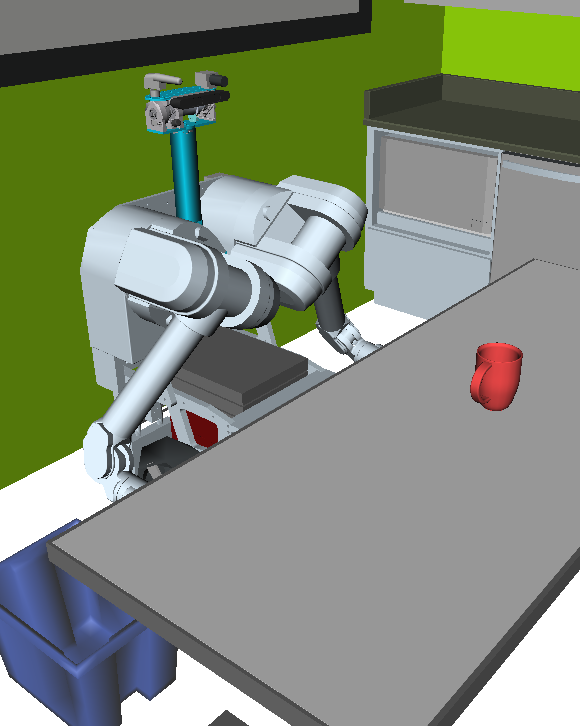
\includegraphics[width=0.185\linewidth]{figs/testherb-a.png}
   }
   \subfloat[Step 1, in $S_{AB}$]{
      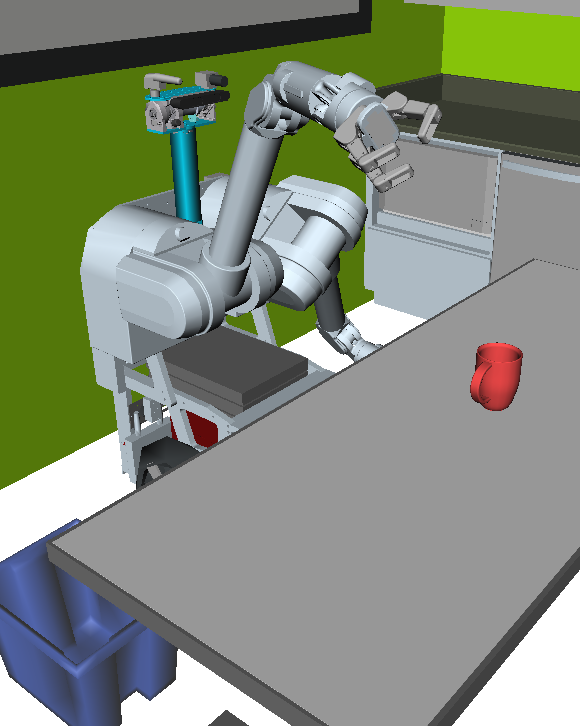
\includegraphics[width=0.185\linewidth]{figs/testherb-b.png}
   }
   \subfloat[Step 2, in $S_{BC}$]{
      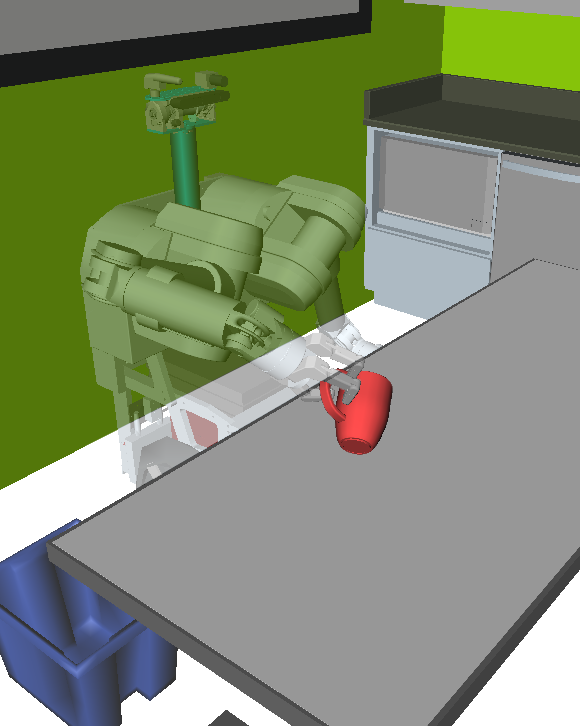
\includegraphics[width=0.185\linewidth]{figs/testherb-c.png}
   }
   \subfloat[Step 3, in $S_{CD}$]{
      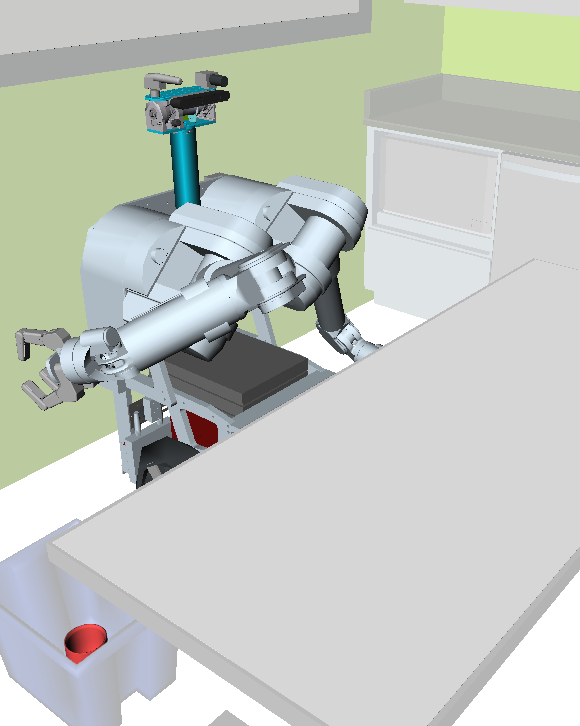
\includegraphics[width=0.185\linewidth]{figs/testherb-d.png}
   }
   \subfloat[Ending Configuration.]{
      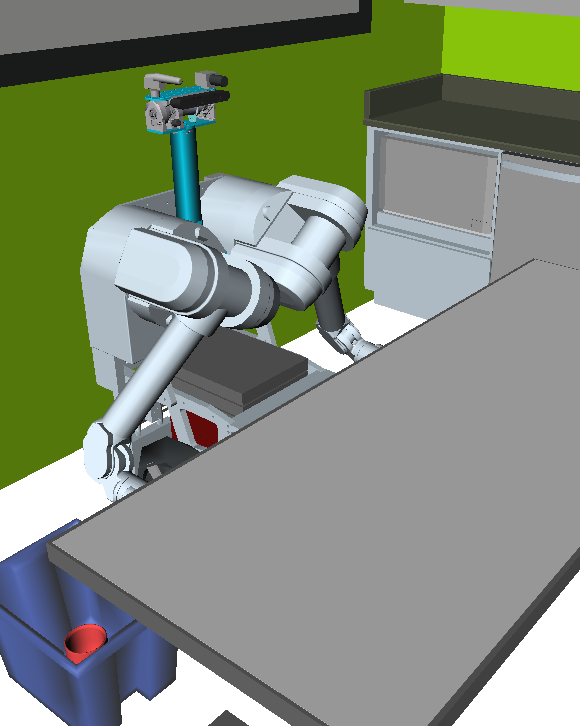
\includegraphics[width=0.185\linewidth]{figs/testherb-e.png}
   }

   \caption[][0.2in]{
     A home robot performing a three-step manipulation task.
     It must move from its home configuration
     to grasp the cup,
     transfer it to a drop location above the bin,
     and return home.}
   \label{fig:family:testherb-problem}
\end{figure*}

The first task we considered is the table clearing task from
Figure~\ref{fig:family:herbbin-multistep-example}.
Each condition for LEMUR was conducted over 50 randomly generated
Halton roadmaps with 10,000 milestones per batch
and a $r_{\ms{loglog}}$ connection radius schedule with $\eta = 1$
(see Section~\ref{sec:roadmaps:roadmap-classes}).
We varied the $\lambda_p$ planning-vs.-execution tradeoff parameter
between $0.0$ to $0.99$ (Chapter~\ref{chap:utility}),
and selected either
the simple edge cost model $\mathcal{M}_{\ms{simple}}$
or the family edge cost model $\mathcal{M}_{\ms{family}}$
described above.

The task consists of 3 steps:
the initial transit to the mug (AB),
the transfer to a drop location (BC),
and the final transit back to the home configuration (CD).
The family module computed a decomposition of the full task
and discovered 7 relevant C-space subsets
over the full planning problem
listed in Table~\ref{table:family:herbbin-subsets}.
An illustration of the subsets is also shown
in Figure~\ref{fig:family:testherb-problem}.

\begin{table*}
   \centering
   \begin{minipage}[t]{.65\textwidth}
   \begin{tabular}{cll}
      \toprule
      Subset & Geometry 1 & Geometry 2 \\
      \midrule
      $S_1$  & RobotMoving & RobotMoving + EnvStatic \\
      $S_2$  & RobotMoving & MugPlacedTable \\
      $S_3$  & RobotMoving & MugPlacedBin \\
      $S_4$  & GraspedMug & RobotMoving + EnvStatic \\
      \bottomrule
   \end{tabular}
   \end{minipage}
   \begin{minipage}[t]{.30\textwidth}
   \begin{tabular}{cl}
      \toprule
      Subset & Defined as \\
      \midrule
      $S_{AB}$  & $S_1 \cap S_2$ \\
      $S_{BC}$  & $S_1 \cap S_4$ \\
      $S_{CD}$  & $S_1 \cap S_3$ \\
      \bottomrule
   \end{tabular}
   \end{minipage}
   \caption[][0.5cm]{Constituent subsets in the \texttt{herbbin} example
      problem.}
   \label{table:family:herbbin-subsets}
\end{table*}

We measured the length of the path returned by each algorithm (rad),
as well as the total planning time as measured by a wall clock (s).

%\begin{figure}
%   \centering
%   \includegraphics{build/multistep-prescribed/herbbin-g1ll}
%   \caption{Example of planning over families for the HERB bin example
%      problem (closest intermediate roots).
%      RRT is red \protect\tikz{\protect\node[fill=red,draw=black]{};}.
%      Individual LEMUR results are dashed
%      (\protect\tikz{\protect\draw[thick,densely dotted] (0,0) -- (0.15,0.15);}),
%      while Family-aware results are solid
%      (\protect\tikz{\protect\draw[thick,solid] (0,0) -- (0.15,0.15);}),.
%      Colors for the inner search algorithm are:
%      \protect\tikz{\protect\node[fill=blue,draw=black]{};}\;IBiD,
%      \protect\tikz{\protect\node[fill=purple,draw=black]{};}\;Heuristic IBiD,
%      and \protect\tikz{\protect\node[fill=olive,draw=black]{};}\;A*.
%      These results use $k_\gamma=1.0$ scaled by $\log(\log(n))/n$.
%      }
%\end{figure}

%\begin{figure}
%   \centering
%   \includegraphics{build/multistep-prescribed/herbbin-r0p9719o}
%   \caption{Example of planning over families for the HERB bin example
%      problem (closest intermediate roots).
%      RRT is red \protect\tikz{\protect\node[fill=red,draw=black]{};}.
%      Individual LEMUR results are dashed
%      (\protect\tikz{\protect\draw[thick,densely dotted] (0,0) -- (0.15,0.15);}),
%      while Family-aware results are solid
%      (\protect\tikz{\protect\draw[thick,solid] (0,0) -- (0.15,0.15);}),.
%      Colors for the inner search algorithm are:
%      \protect\tikz{\protect\node[fill=blue,draw=black]{};}\;IBiD,
%      \protect\tikz{\protect\node[fill=purple,draw=black]{};}\;Heuristic IBiD,
%      and \protect\tikz{\protect\node[fill=olive,draw=black]{};}\;A*.
%      These results use $R=2.0$ scaled by $1/n$.
%      }
%\end{figure}

% nominated intermediate roots!
\begin{figure}
   \centering
   \includegraphics{build/multistep-prescribed/herbbinnom-g1ll}
   \caption[
      Comparison of measured planning time $p$ and solution
      execution cost $x$ for the HERB table-clearing example.
      RRT is shown in red.
      Results for LEMUR with the simple edge cost model are shown in blue,
      while the family edge cost model is shown in green.
      The LEMUR results show the effect of adjusting the $\lambda_p$
      tradeoff parameter from $0$ to $0.99$.
   ]{Comparison of measured planning time $p$ and solution
      execution cost $x$ for the HERB table-clearing example.
      RRT is shown in red \protect\tikz{\protect\node[fill=red,draw=black]{};}.
      Results for LEMUR with the simple edge cost model are shown in
      blue \protect\tikz{\protect\node[fill=blue,draw=black]{};},
      while the family edge cost model is shown in
      green \protect\tikz{\protect\node[fill=green!70!black,draw=black]{};}.
      The LEMUR results show the effect of adjusting the $\lambda_p$
      tradeoff parameter from $0$ (lower right) to $0.99$ (upper left).
      }
\end{figure}

%\begin{figure}
%   \centering
%   \includegraphics{build/multistep-prescribed/herbbinnom-r0p9719o}
%   \caption{Example of planning over families for the HERB bin example
%      problem (nominated intermediate roots).
%      RRT is red \protect\tikz{\protect\node[fill=red,draw=black]{};}.
%      Individual LEMUR results are dashed
%      (\protect\tikz{\protect\draw[thick,densely dotted] (0,0) -- (0.15,0.15);}),
%      while Family-aware results are solid
%      (\protect\tikz{\protect\draw[thick,solid] (0,0) -- (0.15,0.15);}),.
%      Colors for the inner search algorithm are:
%      \protect\tikz{\protect\node[fill=blue,draw=black]{};}\;IBiD,
%      \protect\tikz{\protect\node[fill=purple,draw=black]{};}\;Heuristic IBiD,
%      and \protect\tikz{\protect\node[fill=olive,draw=black]{};}\;A*.
%      These results use $R=2.0$ scaled by $1/n$.
%      }
%\end{figure}

\subsection{Tending a Press Brake with an IRB 4400}

The second task we considered is a sheet metal bending task
using an ABB IRB 4400 robot in an industrial workcell.
See Figure~\ref{fig:family:workcell-configs}
for an illustration of the task.
Each condition for LEMUR was conducted over 50 randomly generated
Halton roadmaps with 10,000 milestones per batch
and a $r_{\ms{loglog}}$ connection radius schedule with $\eta = 1$
(see Section~\ref{sec:roadmaps:roadmap-classes}).
We varied the $\lambda_p$ planning-vs.-execution tradeoff parameter
between $0.0$ to $0.99$ (Chapter~\ref{chap:utility}),
and selected either
the simple edge cost model $\mathcal{M}_{\ms{simple}}$
or the family edge cost model $\mathcal{M}_{\ms{family}}$
described above.

\begin{figure}
   \centering
   \includegraphics{build/workcell/configs}
   \caption{Robot tending a press brake in an industrial workcell.
      This example problem is reproduced from the Lazy PRM paper
      \citep{bohlin2000lazyprm}.
      The multi-step manipulation task requires eight motion planning
      problems in seven different $\mathcal{C}$-subsets.
      From its initial configuration (A),
      the robot moves to grasp a raw sheet (B)
      and transfer first to a settling table (C)
      and subsequently to the press brake (D).
      After the first bend, the robot receives the partially worked
      part (E) and uses a regrasping fixture (F)
      to regrasp it on the other side (G).
      After its second bend (H) and (I),
      the finished part is moved to the final pallet (J)
      before the robot returns to its initial configuration (A).
      Results for planning these steps are shown in
      Figure~\ref{fig:family:workcell-pvx}.}
   \label{fig:family:workcell-configs}
\end{figure}

The task consists of 8 steps,
as described in Figure~\ref{fig:family:workcell-pvx}.
The family module computed a decomposition of the full task
and discovered 17 relevant C-space subsets
over the full planning problem
listed in Table~\ref{table:family:workcell-subsets}.
Note that the motion plans for steps BC and CD are in the same
subset.

\begin{table*}
   \centering
   \begin{minipage}[t]{.65\textwidth}
   \begin{tabular}{cll}
      \toprule
      Subset & Geometry 1 & Geometry 2 \\
      \midrule
      $S_1$  & RobotMoving & RobotMoving + EnvStatic \\
      $S_2$  & RobotMoving & SheetPlacedStart \\
      $S_3$  & RobotMoving & SheetPlacedSettling \\
      $S_4$  & RobotMoving & SheetPlacedDestination \\
      $S_5$  & GraspedTopSide & RobotMoving + EnvStatic \\
      $S_6$  & GraspedTopSide1Flat & RobotMoving + EnvStatic \\
      $S_7$  & GraspedTopSide1Bent & RobotMoving + EnvStatic \\
      $S_8$  & GraspedBotSide & RobotMoving + EnvStatic \\
      $S_9$  & GraspedBotSide2Flat & RobotMoving + EnvStatic \\
      $S_{10}$ & GraspedBotSide2Bent & RobotMoving + EnvStatic \\
      \bottomrule
   \end{tabular}
   \end{minipage}
   \begin{minipage}[t]{.30\textwidth}
   \begin{tabular}{cl}
      \toprule
      Subset & Defined as \\
      \midrule
      $S_{AB}$  & $S_1 \cap S_2$ \\
      $S_{BC}$  & $S_1 \cap S_5 \cap S_6$ \\
      $S_{CD}$  & $S_1 \cap S_5 \cap S_6$ \\
      $S_{EF}$  & $S_1 \cap S_5 \cap S_7$ \\
      $S_{FG}$  & $S_1 \cap S_3$ \\
      $S_{GH}$  & $S_1 \cap S_8 \cap S_9$ \\
      $S_{IJ}$  & $S_1 \cap S_8 \cap S_{10}$ \\
      $S_{JA}$  & $S_1 \cap S_4$ \\
      \bottomrule
   \end{tabular}
   \end{minipage}
   \caption[][0.5cm]{Constituent subsets in the \texttt{workcell} example
      problem.}
   \label{table:family:workcell-subsets}
\end{table*}

We measured the length of the path returned by each algorithm (rad),
as well as the total planning time as measured by a wall clock (s).

\begin{figure}
   \centering
   \includegraphics{build/multistep-prescribed/workcell-g1ll}
   \caption[Comparison of measured planning time $p$ and solution
      execution cost $x$ for the industrial workcell example.
      RRT is shown in red.
      Results for LEMUR with the simple edge cost model are shown in blue,
      while the family edge cost model is shown in green.
      The LEMUR results show the effect of adjusting the $\lambda_p$
      tradeoff parameter from $0$ to $0.99$.
   ]{Comparison of measured planning time $p$ and solution
      execution cost $x$ for the industrial workcell example.
      RRT is shown in red \protect\tikz{\protect\node[fill=red,draw=black]{};}.
      Results for LEMUR with the simple edge cost model are shown in
      blue \protect\tikz{\protect\node[fill=blue,draw=black]{};},
      while the family edge cost model is shown in
      green \protect\tikz{\protect\node[fill=green!70!black,draw=black]{};}.
      The LEMUR results show the effect of adjusting the $\lambda_p$
      tradeoff parameter from $0$ (lower right) to $0.99$ (upper left).
      }
   \label{fig:family:workcell-pvx}
\end{figure}

%\begin{figure}
%   \centering
%   \includegraphics{build/multistep-prescribed/workcell-r1p3128ll}
%   \caption[]{OLD VERSION.
%      Example of planning over families for an industrial
%      workcell example problem.
%      RRT is red \protect\tikz{\protect\node[fill=red,draw=black]{};}.
%      Individual LEMUR results are dashed
%      (\protect\tikz{\protect\draw[thick,densely dotted] (0,0) -- (0.15,0.15);}),
%      while Family-aware results are solid
%      (\protect\tikz{\protect\draw[thick,solid] (0,0) -- (0.15,0.15);}),.
%      Colors for the inner search algorithm are:
%      \protect\tikz{\protect\node[fill=blue,draw=black]{};}\;IBiD,
%      \protect\tikz{\protect\node[fill=purple,draw=black]{};}\;Heuristic IBiD,
%      and \protect\tikz{\protect\node[fill=olive,draw=black]{};}\;A*.
%      These results use $R=2.5$ scaled by $\log(\log(n))/n$.}
%   \label{fig:family:workcell-pvx}
%\end{figure}

%\begin{figure}
%   \centering
%   \includegraphics{build/multistep-prescribed/herbbookshelfnom-g1ll}
%   \caption{Example of planning over families for the HERB bookshelf example
%      problem, with nominated intermediate roots.
%      RRT is red \protect\tikz{\protect\node[fill=red,draw=black]{};}.
%      Individual LEMUR results are dashed
%      (\protect\tikz{\protect\draw[thick,densely dotted] (0,0) -- (0.15,0.15);}),
%      while Family-aware results are solid
%      (\protect\tikz{\protect\draw[thick,solid] (0,0) -- (0.15,0.15);}),.
%      Colors for the inner search algorithm are:
%      \protect\tikz{\protect\node[fill=blue,draw=black]{};}\;IBiD,
%      \protect\tikz{\protect\node[fill=olive,draw=black]{};}\;A*, and
%      \protect\tikz{\protect\node[fill=cyan,draw=black]{};}\;LPA*.
%      These results use $k_\gamma=1.0$ scaled by $\log(\log(n))/n$.
%      }
%\end{figure}

%\begin{figure}
%   \centering
%   \hspace{0.2cm}
%   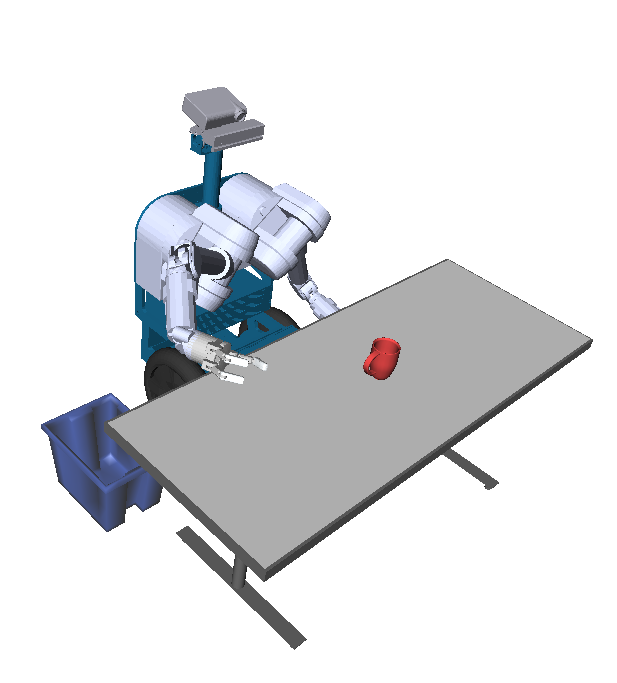
\includegraphics[width=2.7cm]{figs/herbarmmultithread/herbarmmultithread-step0.png}%
%   \;
%   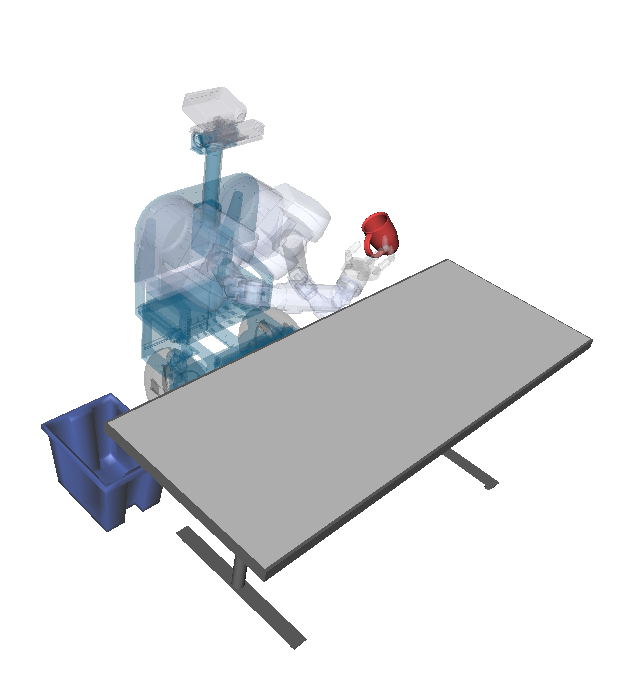
\includegraphics[width=2.7cm]{figs/herbarmmultithread/herbarmmultithread-step1.png}%
%   \;
%   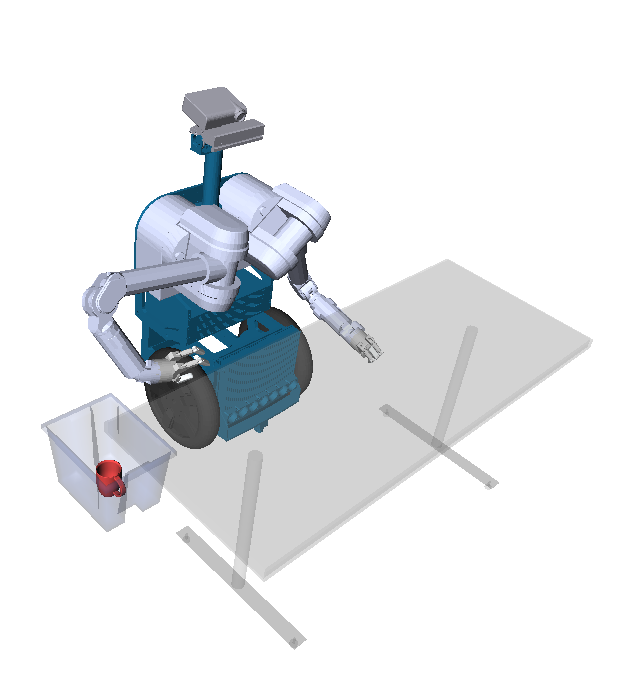
\includegraphics[width=2.7cm]{figs/herbarmmultithread/herbarmmultithread-step2.png}%
%   
%   \includegraphics{build/herbarmmultithread/master-fig}
%   \caption[]{
%      Results from a motion planning experiment for manipulation
%      planning in which the robot must move to grasp the mug
%      and place it into a bin at its side
%      before returning to its initial configuration.
%      In the course of planning the first step to the grasp point,
%      the planner has discovered a number of edges known to be
%      valid.
%      After the grasp, the robot must find a motion to transfer the
%      mug -- any edges known to be valid in the previous step
%      can be used after only checking that the grasped mug does not
%      collide with the environment.
%      Compared with a sequence of single-query calls to LEMUR
%      with model $\mathcal{C}_{\ms{simple}}$
%      \protect\tikz{\protect\node[fill=black!80,draw=black]{};},
%      LEMUR armed with the $\mathcal{M}_{\ms{family}}$ ensemble
%      cost model
%      \protect\tikz{\protect\node[fill=cyan,draw=black]{};}
%      can guide the planner to use edges that are less
%      expensive to validate.}
%   \label{fig:family:herbarmmultithread-master}
%\end{figure}

\section{Implementation Details}

We provide an implementation for the
OpenRAVE \citep{diankov2010openrave}
virtual kinematic planning environment
which automatically discovers $\mathcal{C}$-subsets
in manipulation tasks.

%\cdnote{%
%Special case of this is if objects are disappearing.
%Relation to occupancy grid representations of workspace
%(for deltas, conservative approxs, etc).}

% OTHER POTENTIAL APPLICATIONS:
%
%\subsubsection*{Conservative Bounding Volumes for Different Grasps}
%
%\subsubsection*{Conservative Bounding Volumes for Hypothesized Objects}
%
%There's a sweet ICRA paper here.
%
%\subsubsection*{Dual Arm Stuff}
%
%I think this is related.
%
%Check right arm against gian left side box, etc.
%
%\subsubsection*{Dimensionality Reduction}
%
%The Handey \citep{lozanoperez1987handey} robot
%assumed a box that contained the wrist links at a range of DOF values.
%
%\subsubsection*{Dual-Arm Stuff}
%
%This is very similar to dimensionality reduction.
%
%Loose coupling between arms.
%
%Separate roadmaps for each arm.
%
%Investigate this family structure.
